%\section{Glosario}

%-----------------------construccion glosario--------%

%\makeglossaries

\newglossaryentry{graticula}{ name=grat{\'i}cula , description={
Una grat\'icula es una red de líneas geográficas. Se utiliza esta palabra para referirse a una zona geográfica rectangular, la cual abarca 1º×1º de latitud y longitud. 
}
}

\newglossaryentry{latitud}{ name=Latitud, description={
	Es la distancia angular entre el ecuador y un punto determinado del planeta. La latitud se mide en grados (º), entre 0 y 90; y puede representarse de dos formas:
  \begin{itemize}
\item  indicando a qu\'e hemisferio pertenece la coordenada (norte o sur); 
\item  valores positivos -norte- y negativos -sur-;
  \end{itemize}
as\'i, diez grados en latitud norte podr\'ia representarse 10ºN o 10º; y diez grados sur podr\'ia ser 10ºS o -10º.
En la navegaci\'on mar\'itima la latitud se representa con la letra griega $\phi$.
	}
	 }

\newglossaryentry{statutemile}{ name=Milla estatutaria, description={Llamada simplemente milla, se sigue usando en los países anglosajones y equivale exactamente a 1,609344 km. En inglés se llama statute mile. En los países que utilizan el sistema métrico, la milla aparece normalmente en la escala de los mapas a fin de que éstos puedan ser estudiados también por los anglosajones. De la misma forma, los países anglosajones van incorporando paulatinamente el kil\'ometro como dato adicional en su cartografía. Tiene las siguientes conversiones:
$0.3333$ leguas = $1.609344$ km = 1760 yardas = 5280 pies
}
}

\newglossaryentry{nauticalmile}{ name=Milla n{\'a}utica, description={
	Se introdujo en la náutica hace siglos, y fue adoptada (con muy ligeras variaciones) por todos los países occidentales, siendo definida como la longitud de un arco de 1' de meridiano terrestre. Una milla náutica equivale a 1852 m. Su uso está admitido en el Sistema Internacional (SI).
}
}

\newglossaryentry{nudo}{ name=Nudo, description={
	es una medida de velocidad utilizada tanto para navegación marítima como aérea. Equivale a una milla náutica por hora. También se utiliza en meteorología para medir la velocidad de los vientos. Aunque no existe un símbolo acordado a nivel internacional, tanto la International Hydrographic Organization (IHO) como la Oficina Internacional de Pesas y Medidas (BIPM) recomiendan kn. No obstante, a veces se utilizan kt (knot) para el singular (símbolo de kilotonelada) y kts para el plural.
}
}


\newglossaryentry{actitud}{name=Actitud, description={
 Respecto a una aeronave se define como los \'angulos que su nariz y alas forman con la referencia que es el horizonte. De esa manera hablamos de actitud nariz arriba, ala izquierda abajo, etc.
}
}


\newglossaryentry{longitud}{ name=Longitud, description={
Expresa la distancia angular entre un punto dado de la superficie terrestre y el meridiano que se tome como 0º; habitualmente en la actualidad el meridiano de Greenwich (observatorio de Greenwich), pero antiguamente hubo muchos otros que serv\'ian como referencia (para el mapa de Ptolomeo el meridiano de Alejandr\'ia, para los mapas espa\~noles hasta el siglo XIX el meridiano de C\'adiz -observatorio de C\'adiz- o el meridiano de Salamanca -observatorio de la Universidad de Salamanca, utilizado por la Compa\~n\'ia de Jes\'us-, para los franceses el meridiano de Par\'is -observatorio de Par\'is-, etc.).
La longitud geogr\'afica se mide en grados (º). Existen varias maneras de medirla y expresarla:
\begin{itemize}
\item  entre 0º y 360º, aumentando hacia el Este del meridiano 0º
\item  entre 0º y 180º indicando a qu\'e hemisferio pertenece
\item entre 0º y   180º positivos -Este- o negativos -Oeste-;
\end{itemize}
as\'i, noventa grados longitud este puede representarse 90º o 90ºE; y noventa grados Oeste puede ser 270º, 90ºO o -90º
En navegaci\'on mar\'itima la longitud se representa con la letra griega $\omega$.
	}
	 }

\newglossaryentry{trayectoria}{ name=Trayectoria, description={
Se define como el conjunto de puntos del espacio por los cuales pasa la aeronave durante su vuelo %(ver Figura \ref{fig:trayectoria}).
}
}

\newglossaryentry{proyeccion-cartografica}{ name=Proyecci{\'o}n cartogr{\'a}fica, description={
 La representación de la superficie de referencia (esfera o elipsoide de revolución) sobre una superficie plana, sin que haya deformaciones es geométricamente imposible. Se producen deformaciones de tipo angular, lineal y superficial al representar en un plano la superficie terrestre.
En cartografía, este problema se resuelve mediante las proyecciones cartográficas.
La proyección cartográfica consiste en la correspondencia biunívoca entre los puntos de la superficie de referencia y sus transformaciones en el plano, llamado plano de proyección con deformaciones controladas. 
\begin{figure}[!h]
  \centering
  \subfigure[Concepto de proyecci\'on]{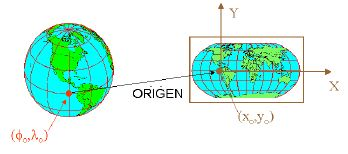
\includegraphics[width=0.5\textwidth]{./Imagenes/transformacion.JPG}}
  \subfigure[Tipos de proyecciones]{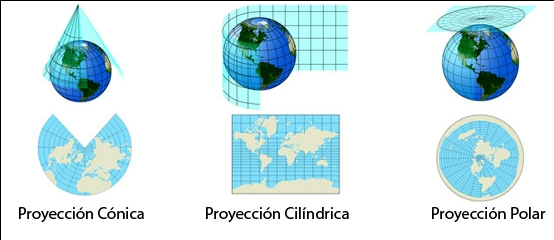
\includegraphics[width=0.5\textwidth]{./Imagenes/proyecciones}}
  \caption{Proyecciones cartogr\'aficas}
  \label{fig:proyecciones.cartograficas}
\end{figure}
}
}

%\begin{description}


% \item [Longitud] Expresa la distancia angular entre un punto dado de la superficie terrestre y el meridiano que se tome como 0º; habitualmente en la actualidad el meridiano de Greenwich (observatorio de Greenwich), pero antiguamente hubo muchos otros que serv\'ian como referencia (para el mapa de Ptolomeo el meridiano de Alejandr\'ia, para los mapas espa\~noles hasta el siglo XIX el meridiano de C\'adiz -observatorio de C\'adiz- o el meridiano de Salamanca -observatorio de la Universidad de Salamanca, utilizado por la Compa\~n\'ia de Jes\'us-, para los franceses el meridiano de Par\'is -observatorio de Par\'is-, etc.).
% La longitud geogr\'afica se mide en grados (º). Existen varias maneras de medirla y expresarla:

% \begin{itemize}
% \item  entre 0º y 360º, aumentando hacia el Este del meridiano 0º

% \item  entre 0º y 180º indicando a qu\'e hemisferio pertenece

% \item entre 0º y   180º positivos -Este- o negativos -Oeste-;
% \end{itemize}

% as\'i, noventa grados longitud este puede representarse 90º o 90ºE; y noventa grados Oeste puede ser 270º, 90ºO o -90º
% En navegaci\'on mar\'itima la longitud se representa con la letra griega $\omega$.

% \item [Actitud de una aeronave] Se define como los \'angulos que su nariz y alas forman con la referencia que es el horizonte. De esa manera hablamos de actitud nariz arriba, ala izquierda abajo, etc.

% \item [Marco de coordenadas de referencia] Define un punto de origen y un conjunto de ejes que parten de dicho origen con una determinada orientaci\'on. Estos ejes son los llamados ejes de coordenadas. Los marcos de referencia pueden o no ser inerciales. Se habla de un marco de referencia inercial si \'este no est\'a sujeto a aceleraciones, encontr\'andose en reposo o en movimiento traslacional uniforme. En los marcos de referencia inerciales se pueden aplicar las leyes de la mec\'anica de Newton.

% \item [Posici\'on] Es el conjunto de coordenadas que identifica a un punto dado en un marco de coordenadas espec\'ifico. El proceso para hallar la posici\'on a menudo es llamado posicionamiento.

% \item [Enrutamiento] Se denomina as\'i al proceso de planificar la ruta adecuada para llegar al destino.

% \item [Guiado] Este es el procedimiento para que un veh\'iculo siga por la ruta predefinida.

% \item [Trayectoria] Se define como el conjunto de puntos del espacio por los cuales pasa la aeronave durante su vuelo (ver Figura \ref{fig:trayectoria}).

% \item [Ruta] Es la curva resultante de proyectar la trayectoria sobre la superficie de la Tierra (ver Figura \ref{fig:trayectoria}).

% \item [Waypoints] Son puntos conocidos a lo largo de la ruta, y a menudo resaltan por alguna raz\'on en particular (Lugares de reporte obligatorio, puntos de intersecci\'on de aerov\'ias, etc.) (ver Figura \ref{fig:trayectoria}).

% \item [Tramo] Llamado en ingl\'es ``\textit{leg}'' (pierna), se define como un segmento de ruta comprendido entre dos waypoints (ver Figura \ref{fig:trayectoria}). 

% \item [Curso deseado] Es el \'angulo entre el norte (cualquiera que se est\'e usando: magn\'etico, geogr\'afico, etc) y la l\'inea recta que une dos waypoints sucesivos en la ruta. En ingl\'es se denomina ``\textit{Desired Track}'', y se abrevia DTK (ver Figura \ref{fig:curso}).

% \item [Derrota] En n\'autica, la derrota es el trayecto que ha recorrido una embarcaci\'on desde un punto ``\textit{A}'' hasta otro punto ``\textit{B}''. En el derrotero o carta n\'autica se traza la ruta a seguir; contiene informaciones importantes para el navegante, tales como ubicaci\'on de faros, boyas, profundidad del agua, etc. En navegaci\'on a\'erea es el \'angulo entre el norte y la l\'inea tangente a la ruta (dicha tangente corresponde, por cierto, al vector velocidad de la aeronave). En ingl\'es se le llama ``\textit{Track}'' o TK (ver Figura \ref{fig:curso}).

% \item [Error transversal] El error transversal o ``\textit{Cross-Track Error}'' (XTE) es la distancia perpendicular entre la posici\'on de la aeronave y la l\'inea que representa al curso deseado. \footnote{Es conveniente tener en cuenta que la diferencia entre el curso deseado (DTK) y la ruta realmente seguida (TK) por lo general es producida por factores externos tales como el viento cruzado (en el caso de las aeronaves) o las corrientes marinas (si se habla de barcos).}

% \item [Rumbo] El rumbo o ``Heading'' (HDG) es el \'angulo entre el norte y el eje longitudinal de la aeronave (hacia donde apunta su nariz). No coincide necesariamente con el vector velocidad (Track) dado que es posible, por ejemplo, que el piloto modifique el rumbo para contrarestar un viento cruzado (ver Figura \ref{fig:curso}).

% \item [Marcaci\'on] Se define como el \'angulo entre el norte y la l\'inea recta que une a un punto de referencia dado con la aeronave. A menudo, el punto de referencia coincide con alguna instalaci\'on importante en tierra tal como una radioayuda. En ingl\'es se le llama ``\textit{Bearing}''. Notese que el ``\textit{bearing}'' depender\'a siempre del punto que se est\'e tomando como referencia (ver Figura \ref{fig:curso}). 

% \item [ETE] ``\textit{Estimated Time En-route}'', es el intervalo de tiempo estimado que tardar\'a la aeronave en su ruta desde el punto de origen hasta el punto de destino.

% \item [ETA] ``\textit{Estimated Time of Arrival}'', es la hora estimada en que la aeronave llegar\'a a su punto de destino propuesto. 

% \item [Norte] El aparentemente simple concepto de ``\textit{Norte}'' engloba una serie de definiciones que es necesario conocer y diferenciar adecuadamente: 

%    \begin{description}
%      \item [Norte geogr\'afico] Es el que viene dado por la intersecci\'on del eje de rotaci\'on de la Tierra con la superficie de la misma 1.1. Es llamado tambi\'en ``\textit{Norte verdadero}'', y en \'el confluyen todos los meridianos.

% \item [Norte magn\'etico] Es el punto donde la mayor parte de las l\'ineas de fuerza del campo magn\'etico terrestre entran en la superficie. Se puede detectar utilizando instrumentos tales como la br\'ujula y la ``\textit{flux valve}'' (equivalente a la br\'ujula en las aeronaves modernas).

% Es importante hacer notar que el norte geogr\'afico y el magn\'etico \textbf{NO} coinciden, y que adem\'as el norte magn\'etico cambia su posici\'on con el tiempo.

% \item [Declinaci\'on magn\'etica] es el \'angulo de desviaci\'on entre las posiciones del norte magn\'etico y geogr\'afico, vistas desde un punto en particular. Se denota como D y se considera positiva cuando el \'angulo medido est\'a hacia el Este del norte verdadero, y negativo en caso contrario (ver Figura \ref{fig:declinacion-magnetica}). 

% \item [L\'ineas is\'ogonas] Se llaman as\'i a las l\'ineas que, sobre las cartas de navegaci\'on o los mapas, unen puntos que tienen la misma declinaci\'on magn\'etica. Son tambi\'en denominadas l\'ineas isog\'onicas. Adicionalmente, si una l\'inea corresponde a puntos con declinaci\'on 0º, se habla de l\'inea ag\'onica. En la Figura \ref{fig:declinacion-magnetica-anio-2000} se presenta un mapa mundial con los valores de la declinaci\'on magn\'etica para el a\~no 2000.

% \item [Norte de la Br\'ujula] Es el norte magn\'etico tal y como lo indica a bordo el instrumento adecuado (br\'ujula o flux valve). No indica realmente el norte magn\'etico pues el instrumento comete errores por diversas razones (presencia de masas met\'alicas cercanas, l\'ineas de campo magn\'etico que no son horizontales, etc).

% \item [Desviaci\'on magn\'etica] Es el error angular cometido por la br\'ujula o flux valve. El fabricante de la aeronave puede corregirla hasta cierto punto. En la Figura \ref{fig:declinacion-desviacion} se presenta la relaci\'on entre los nortes geogr\'afico, magn\'etico y de la br\'ujula con sus correspondientes diferencias angulares. 

% \item [Norte de la Cuadr\'icula] Cuando se navega a grandes latitudes (muy al norte o muy al sur del planeta), no tiene sentido guiarse por el norte magn\'etico debido, entre otras cosas, a las grandes declinaciones implicadas. Es por ello que se define arbitrariamente el Norte de la Cuadr\'icula como el norte indicado por los meridianos de la carta de navegaci\'on que se est\'a usando para navegar. 

%    \end{description}

% \item [Navegaci\'on por estima] Llamada en ingl\'es \textit{dead reckoning}, representa el proceso mediante el cual, a partir de una posici\'on previa bien conocida (llamada fix), y estimando el vector velocidad de la aeronave y el tiempo transcurrido, se obtiene (por integraci\'on en funci\'on del tiempo) la posici\'on actual de la aeronave (ver Figura \ref{fig:dead-reckoning}). 

% \end{description}



